% Template taken with permission from Richard Hu
% Modified by Rahul Shah
% Last Updated: 2021-02-06 21:25

\documentclass[11pt]{article}
\usepackage{header}
\usepackage{mathrsfs}
\usepackage{mdframed}
\usepackage{pdfpages}
\usepackage{titlesec}

\newmdenv[%
    leftmargin=-5pt,
    rightmargin=-5pt, 
    innerleftmargin=5pt,
    innerrightmargin=5pt,
    backgroundcolor=brown!10,
]{Answer}%
\def\title{Homework 04}

\def\R{\mathbb{R}} % Real Numbers
\def\P{\mathbb{P}}
\def\A{\textbf{A}} % Bold matrices
\def\B{\textbf{B}}
\def\AB{\textbf{AB}}
\def\BA{\textbf{BA}}
\newcommand{\pd}[2]{\frac{\partial{#1}}{\partial{#2}}}
\let\originalmiddle=\middle
\def\middle#1{\mathrel{}\originalmiddle#1\mathrel{}}
\newcommand\aug{\fboxsep=-\fboxrule\!\!\!\fbox{\strut}\!\!\!}


\makeatletter
\newcount\my@repeat@count
\newcommand{\myrepeat}[2]{%
  \begingroup
  \my@repeat@count=\z@
  \@whilenum\my@repeat@count<#1\do{#2\advance\my@repeat@count\@ne}%
  \endgroup
}
\makeatother

\titlelabel{\thetitle.\enspace}


\begin{document}
\maketitle
\fontsize{12}{15}\selectfont

\begin{center}
    HW Due: February 12, 2021, at 23:59 \\
    Self-grades due: February 15, 2021, at 23:59
\end{center}

    \begin{enumerate}
        \item $\textbf{Exam Policy and Practice}$
        \begin{enumerate}
            \item Please read through the entirety of the \href{https://docs.google.com/document/d/10pnWwxyZ40nlpbCM4aOYTxXOjc36sIQaMx9m8zyaR8w/edit?usp=sharing}{EECS 16A exam proctoring policies} carefully before proceeding.
            \\
            This question is designed to familiarize you with how the exam will be run and help you setup and practice.
             \begin{enumerate}
               \item If you experience no disruptions during the exam, how many total minutes do you have for scanning and submission? What if there is a disruption?
               \begin{Answer}
               \end{Answer}
               \item Are you required to record locally during the exam? How much space should you have available on your computer for a local recording?
               \begin{Answer}
               \end{Answer}
               \item How should you contact the course staff in case of an emergency situation during the exam?
               \begin{Answer}
               \end{Answer}
             \end{enumerate}
             \item Please configure your Zoom link.
             \begin{enumerate}
               \item \href{https://forms.gle/P53yLvoxnW8j672W9}{https://forms.gle/P53yLvoxnW8j672W9}
               \begin{Answer}
               \end{Answer}
             \end{enumerate}
             \item Practice Zoom Recording 
             \begin{enumerate}
               \item \href{https://forms.gle/21MaHrjyTEVMBenQ8}{https://forms.gle/21MaHrjyTEVMBenQ8}
               \begin{Answer}
               \end{Answer}
             \end{enumerate}
           \end{enumerate}
    
   \newpage
   \item $\textbf{Reading Assignment}$
       \begin{enumerate}
           \item how you can use the strategies in the notes to tackle proof questions
           \begin{Answer}
                Answer part a here
            \end{Answer}
           \item how we can interpret the rows and columns of a state transition matrix
           \begin{Answer}
                Answer part b here
           \end{Answer}
       \end{enumerate}
       
   \newpage
   \item $\textbf{Multiply the Matrices}$
       \begin{enumerate}
           \item We have two matrices $\A$ and $\B$, where $\A$ is a $3\times2$ matrix and $\B$ is a $2\times 4$ matrix. Would the multiplication $\AB$ be a valid operation? If yes, what do you expect the dimensions of $\AB$ to be?
           \begin{Answer}
                Answer part a here
            \end{Answer}
           \item Compute $\AB$ by hand, where $\A$ and $\B$ are given by
                \[
                    \A = \begin{bmatrix}
                        1 & 0 \\
                        2 & 1 \\
                        0 & 1
                    \end{bmatrix}, 
                    \land \qquad
                    \B = \begin{bmatrix}
                            1  & 2 & -1 & 0 \\
                            -3 & 0 & 2  & -1
                    \end{bmatrix}
                \]
            Compute $\BA$ too if the operation is valid. If it is invalid, explain why. Make sure you show the work for your calculations.
           \begin{Answer}
                Answer part b here
           \end{Answer}
           \item Now let us assume $\A  \R^{2\times n}$ is a \textbf{new matrix with 2 rows}, which are given by the \textbf{transpose}s of column vectors $\vec r_1, \vec r_2$ i.e
           \[
                    \A = \begin{bmatrix}
                        - & \vec r_1^T & - \\
                        - & \vec r_2^T & -
                        \end{bmatrix},
                    \qquad 
                    \text{where}, 
                    \qquad
                    \vec r_1 = \begin{bmatrix}
                                r_{11} \\
                                r_{12} \\
                                \vdots \\
                                r_{1n}
                    \end{bmatrix},
                    \text{ and}
                    \qquad
                    \vec r_2 = \begin{bmatrix}
                                r_{21} \\
                                r_{22} \\
                                \vdots \\
                                r_{2n}
                    \end{bmatrix}.
                \]
                $\B \in \R^{n\times 3}$ is a new matrix with 3 columns, which are called $\vec c_1, \vec c_2,\text{ and }\vec c_3,$ i.e.
                \[
                    \B = \begin{bmatrix}
                            \mid & \mid & \mid \\
                            \vec c_1 & \vec c_2 & \vec c_3 \\
                            \mid & \mid & \mid
                         \end{bmatrix},
                         \qquad 
                        \text{where}, 
                        \qquad
                        \vec c_1 = \begin{bmatrix}
                                    c_{11} \\
                                    c_{12} \\
                                    \vdots \\
                                    c_{1n}
                        \end{bmatrix},
                        \vec c_2 = \begin{bmatrix}
                                    c_{21} \\
                                    c_{22} \\
                                    \vdots \\
                                    c_{2n}
                        \end{bmatrix},
                        \text{ and}
                        \qquad
                        \vec c_3 = \begin{bmatrix}
                                    c_{31} \\
                                    c_{32} \\
                                    \vdots \\
                                    c_{3n}
                        \end{bmatrix}.
                \]
                Now show that:
$\AB = \begin{bmatrix}
    \vec r_1^T \vec c_1 & \vec r_1^T \vec c_2 & \vec r_1^T \vec c_3 \\
    \vec r_2^T \vec c_1 & \vec r_2^T \vec c_2 & \vec r_2^T \vec c_3
\end{bmatrix}$ if $\AB$ is a valid operation.
        \begin{Answer}
            Answer here.
        \end{Answer}
       \end{enumerate}
   
   \newpage
   \item $\textbf{Linear Dependence in a Square Matrix}$
   Let $A$ be a square $n\times n$ matrix, (i.e. both the columns and rows are vectors in $\R^n$). Suppose we are told that the columns of A are linearly dependent. Prove, then, that the rows of A must also be linearly dependent.
   \\
    You can use the following conclusion in your proof:
    \\
    \textit{If Gaussian elimination is applied to a matrix A, and the resulting matrix (in reduced row echelon form) has at least one row of all zeros, this means that the rows of A are linearly dependent.}
    
    (Hint: Can you use the linear dependence of the columns to say something about the number of solutions
    to $\A\vec x =\vec 0$? How does the number of solutions relate to the result of Gaussian elimination?)
    \begin{Answer}
        ..
    \end{Answer}

   \newpage
   \item $\textbf{Kinematic Model for a Simple Car}$
   \begin{enumerate}
       \item We assume that the car has a small heading, $\theta$, which is a \textbf{very small but nonzero }value, and that the steering angle $\phi$ is also \textbf{very small but nonzero}. In this case, we could use the following approximations:
        \begin{gather*}
            \sin{\alpha} \approx 0,
            \\
            \cos{\alpha} \approx 1,
            \\
            \tan{\alpha} \approx 0.
        \end{gather*}
        where $\alpha$ is the small angle of interest, and $\approx$ means "approximately equal to". Here, we use a very simple approximation for small angles; in later classes, you may learn better approximations. 
        \\
        Draw, by hand, graphs of $\sin(\alpha)$ and $\cos(\alpha)$, for $\alpha$ ranging from $-\pi$ to $\pi$. Using these graphs can you justify the approximation we are making for small values of $\alpha$?
        \begin{Answer}
            ..
        \end{Answer}

        
        
        % attach the others via pdf
        
        % TODO: upload your own my_ipyntbk.pdf 
        % 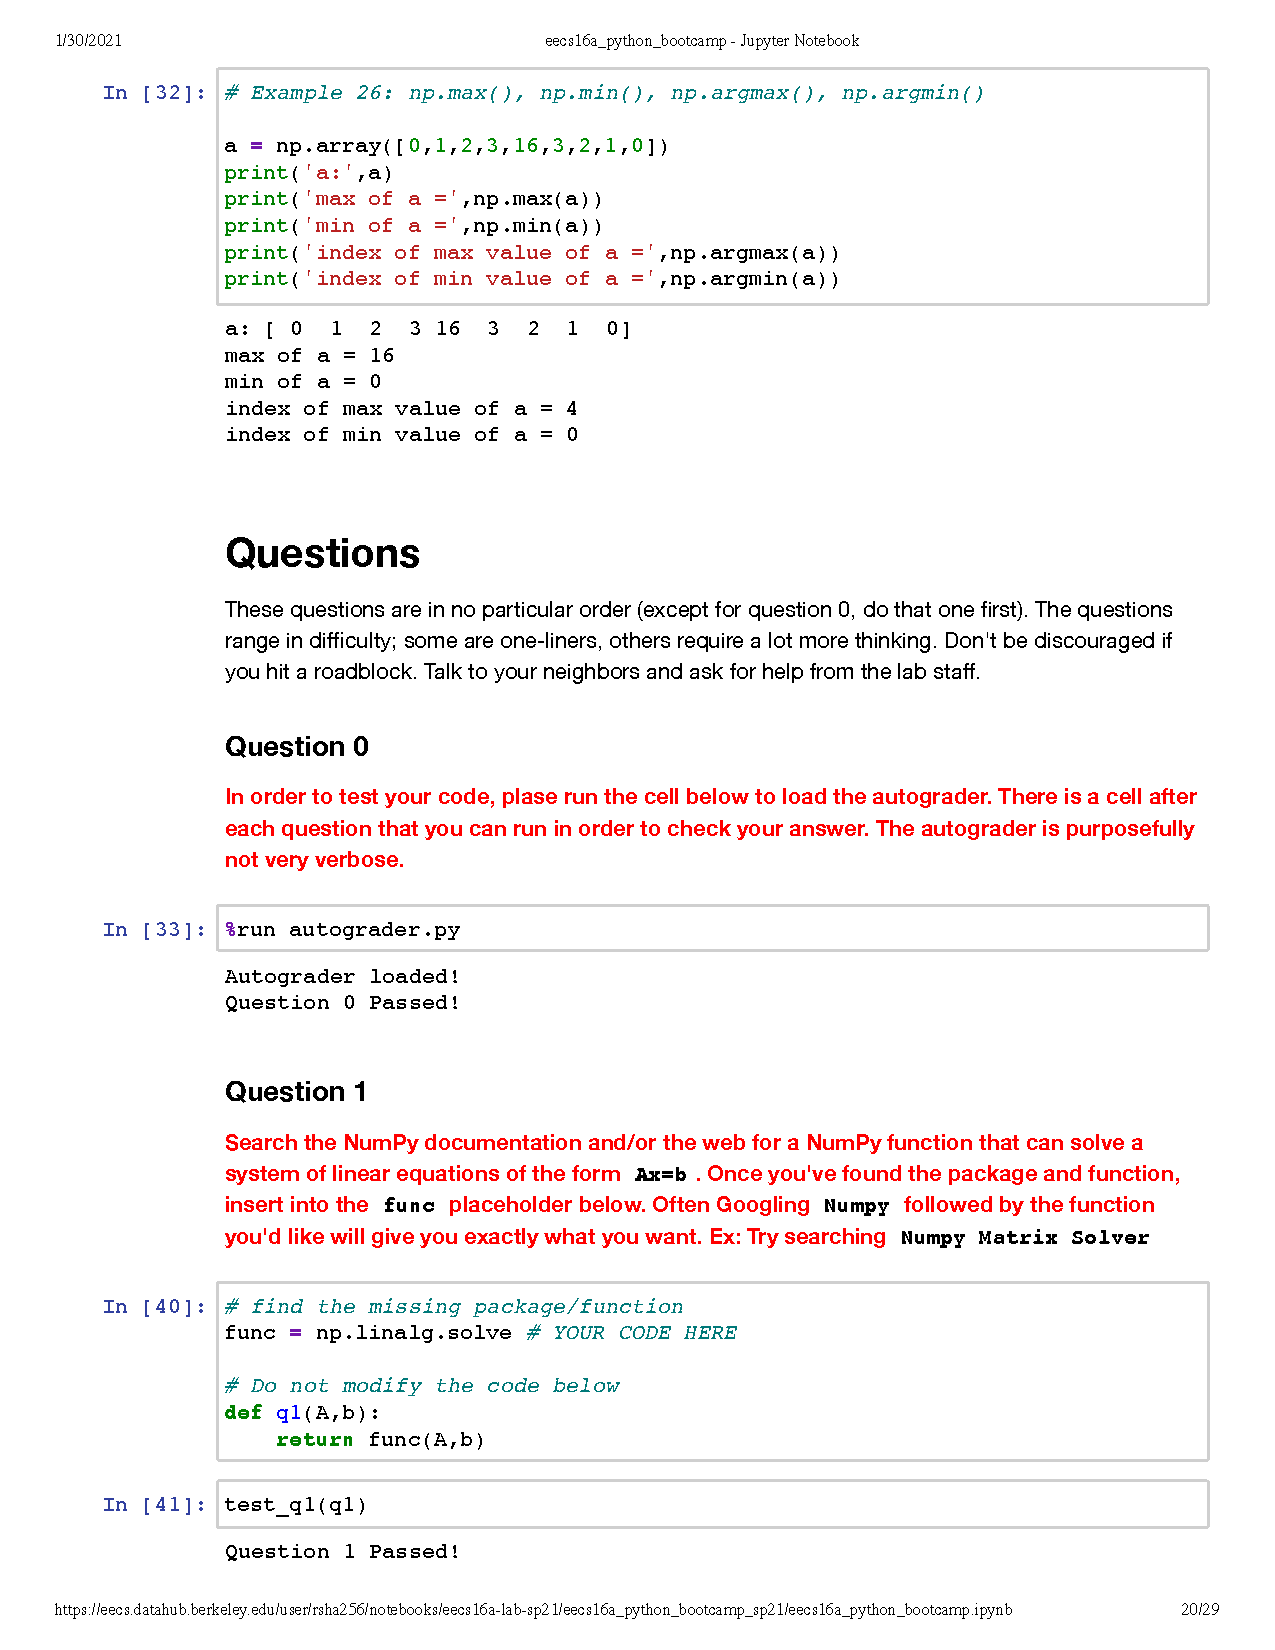
\includepdf[pages=-, noautoscale=true, scale=.8]{my_ipyntbk.pdf} 
        
        % TODO: upload your own my_ipyntbk.pdf 
        % 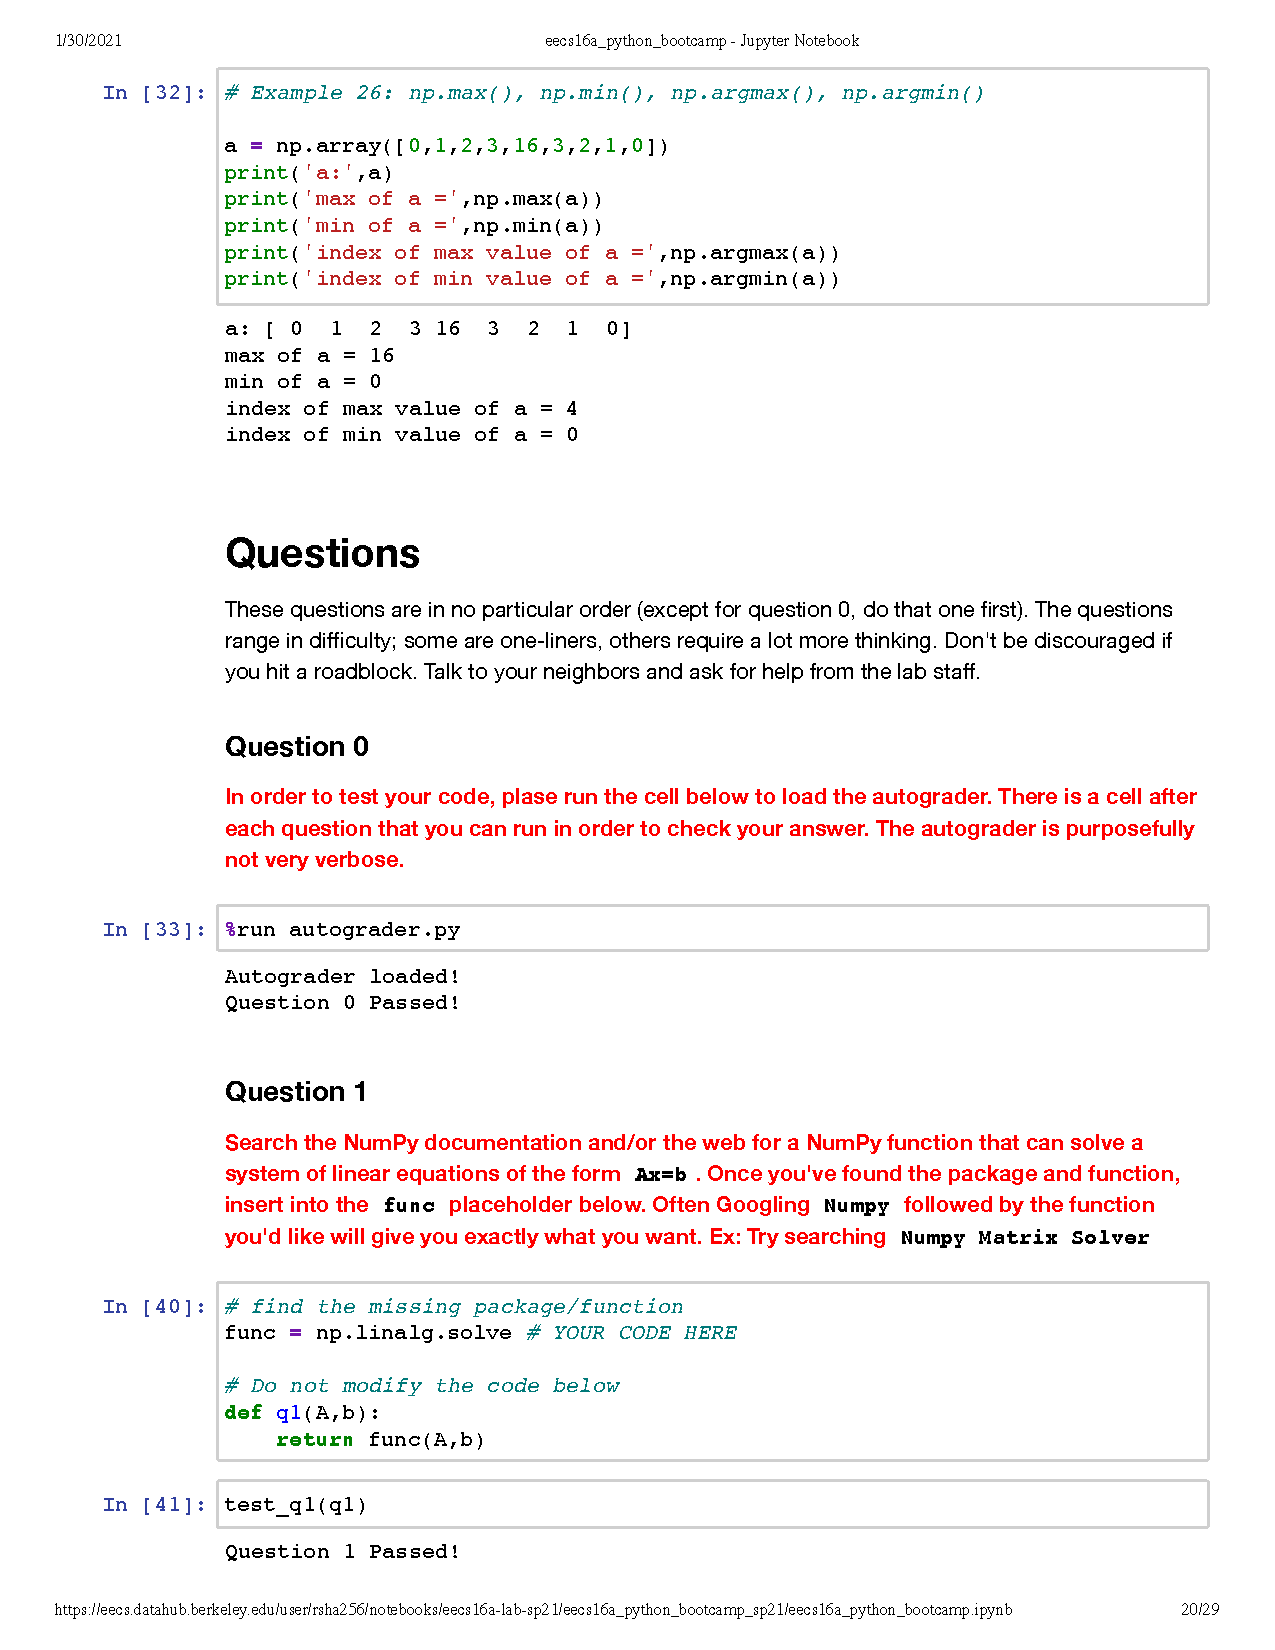
\includepdf[pages=-, noautoscale=true, scale=.8]{my_ipyntbk.pdf} 
        
        % TODO: upload your own my_ipyntbk.pdf 
        % 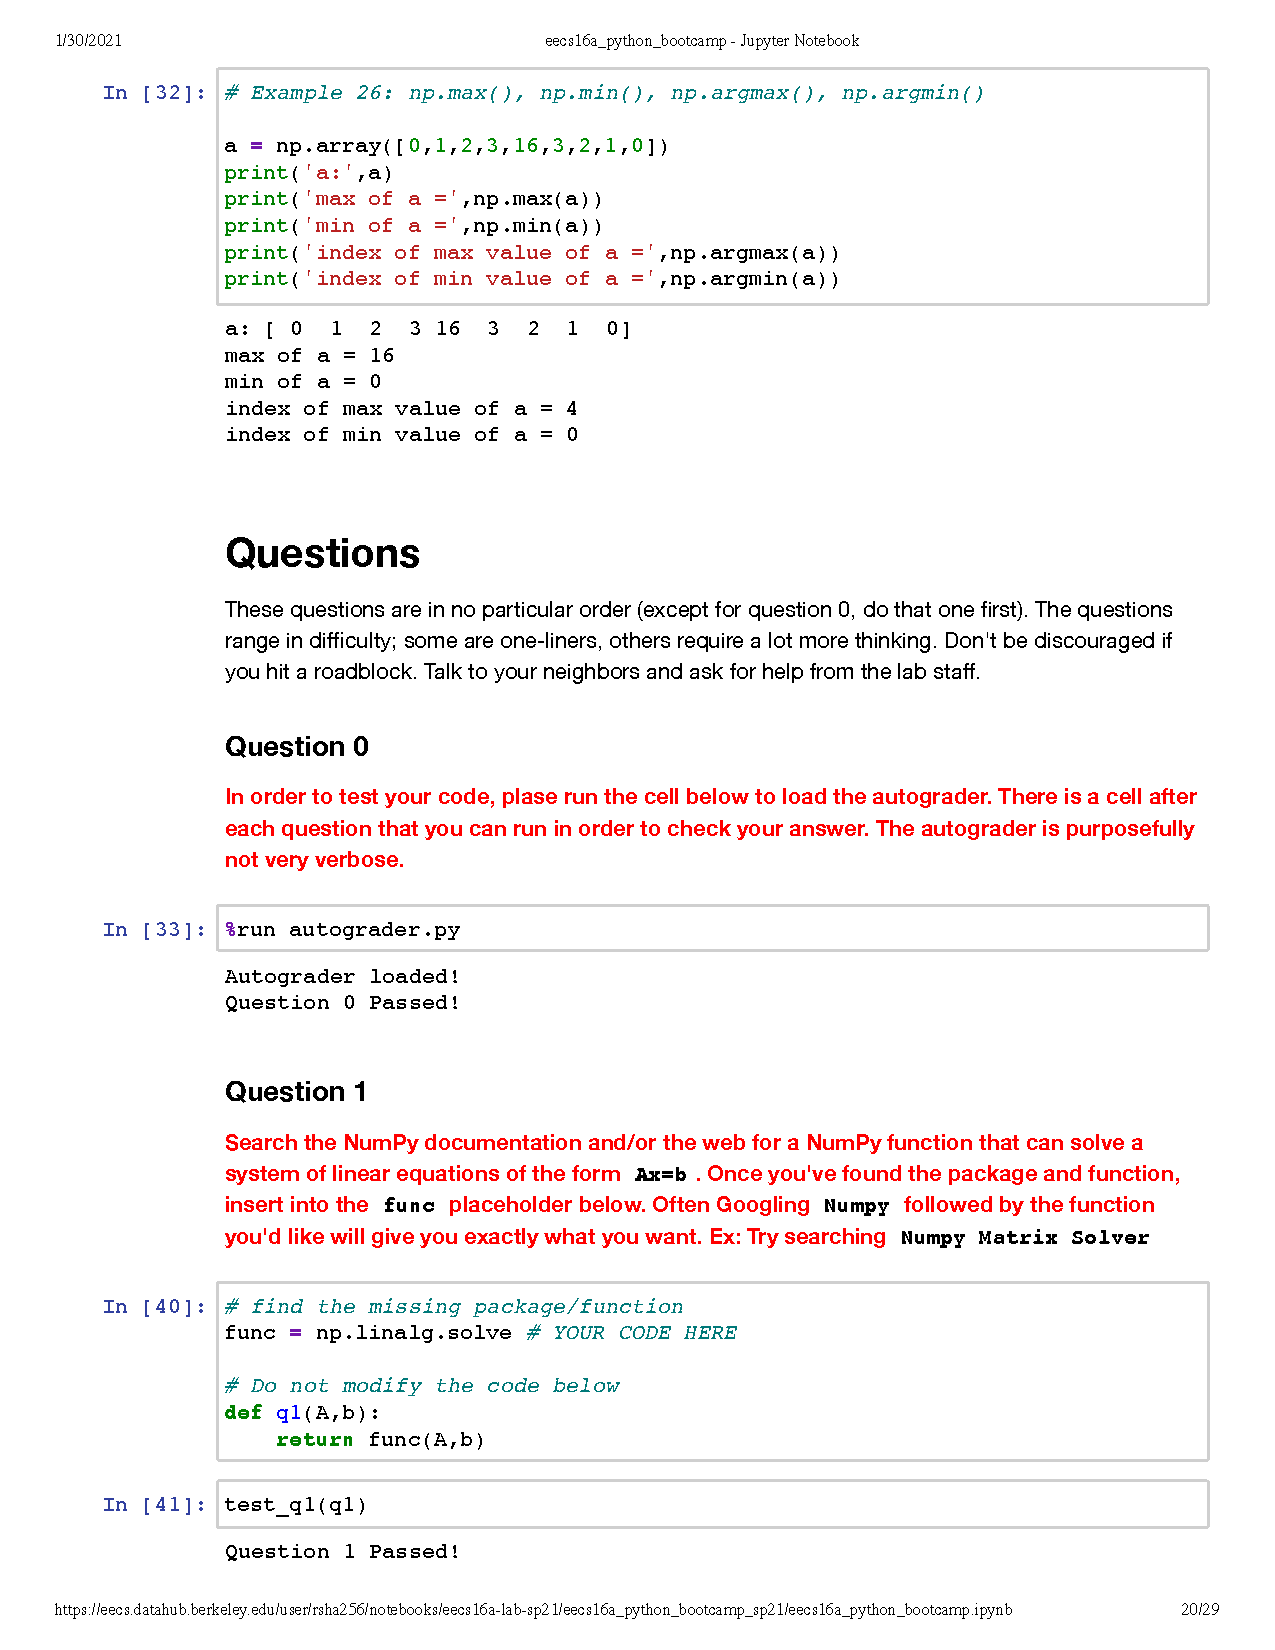
\includepdf[pages=-, noautoscale=true, scale=.8]{my_ipyntbk.pdf} 
   \end{enumerate}
   \newpage
   \item $\textbf{Image Stitching}$
       \begin{enumerate}
           \item To understand how the matrix \textbf{R} and vector $\vec t$ transforms any vector representing a point on a image,
            Consider this equation similar to Equation (5),
                \[
                	\vec v = \begin{bmatrix}
                    		    2 & 2 \\
                			   -2 & 2
                	\end{bmatrix} \vec u + \vec w 
                    = \vec v_1 + \vec w.
                \]
                Use $\vec w = \begin{bmatrix}
                				0 \\
                				1
                            \end{bmatrix},
                    $
                    $\vec u = \begin{bmatrix}
                				1 \\
                				1
                            \end{bmatrix},$
                            for this part.
                We want to find out what geometric transformation(s) can be applied on $\vec u$ to give $\vec v$.
                \begin{Answer}
                    ...
                \end{Answer}
                
            \item Multiply Equation (5) out into two scalar linear equations.
            \begin{enumerate}
                \item What are the known values and what are the unknowns in each equation?
                    \begin{Answer}
                        .
                    \end{Answer}
                \item How many unknowns are there?
                    \begin{Answer}
                        ..
                    \end{Answer}
                \item How many independent equations do you need to solve for all the unknowns?
                    \begin{Answer}
                        ...
                    \end{Answer}
                \item How many pairs of common points ~p and ~q will you need in order to write down a system of equations that you can use to solve for the unknowns?
                    \begin{Answer}
                        ....
                    \end{Answer}
            \end{enumerate}
            
            \item Write out a system of linear equations that you can use to solve for $\alpha = \begin{bmatrix}
                                    r_{xx} \\
                                    r_{xy} \\
                                    r_{yx} \\
                                    r_{yy} \\
                                    r_{t_x} \\
                                    r_{t_y}
                                \end{bmatrix}
                    $. Assume that all four pairs of points from Fig. 4 are labeled as:
                    \[
                        \begin{aligned}
                            \vec q_1 = \begin{bmatrix}
                                            q_{1x} \\
                                            q_{1y}
                                       \end{bmatrix},
                            \vec p_1 = \begin{bmatrix}
                                            p_{1x} \\
                                            p_{1y}
                                       \end{bmatrix} \
                            \vec q_1 = \begin{bmatrix}
                                            q_{2x} \\
                                            q_{2y}
                                       \end{bmatrix},
                              \vec p_1 = \begin{bmatrix}
                                            p_{2x} \\
                                            p_{2y}
                                       \end{bmatrix} \
                              \vec q_1 = \begin{bmatrix}
                                            q_{3x} \\
                                            q_{3y}
                                       \end{bmatrix},
                              \vec p_1 = \begin{bmatrix}
                                            p_{3x} \\
                                            p_{3y}
                                       \end{bmatrix} \
                              \vec q_1 = \begin{bmatrix}
                                            q_{4x} \\
                                            q_{4y}
                                       \end{bmatrix},
                              \vec p_1 = \begin{bmatrix}
                                            p_{4x} \\
                                            p_{4y}
                                       \end{bmatrix}.
                        \end{aligned}\]
                Now think of your answer to Part b(iv). How many pairs of these points would you need to solve for
                $\vec \alpha$. Choose just enough equations required to solve for $\vec \alpha$ and express these linear equations using
                matrix-vector form.
                \begin{Answer}
                        ...
                \end{Answer}
       \end{enumerate}
   
   % TODO: upload your own my_ipyntbk.pdf 
        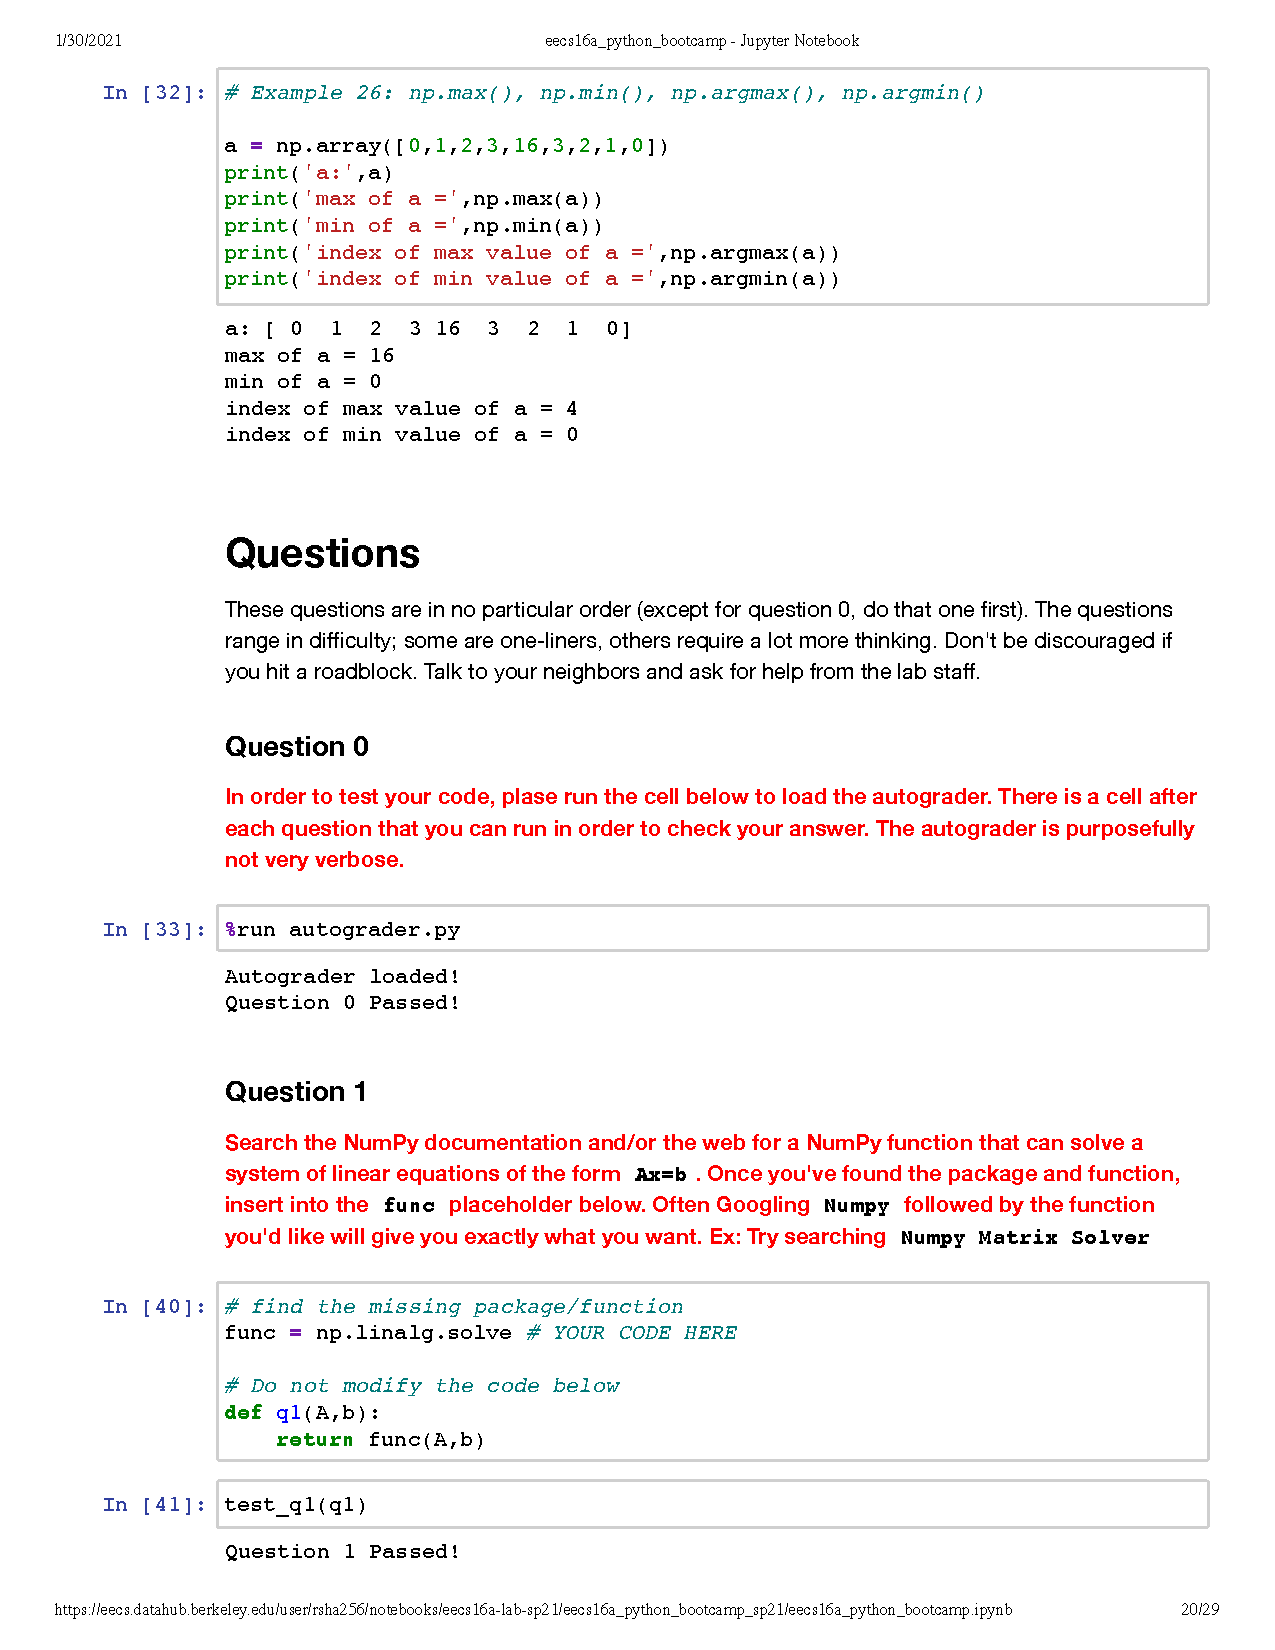
\includepdf[pages=-, noautoscale=true, scale=.8]{my_ipyntbk.pdf} 
   
   \newpage
   \item $\textbf{Social Media}$
       \begin{figure}[h]
        \centering
        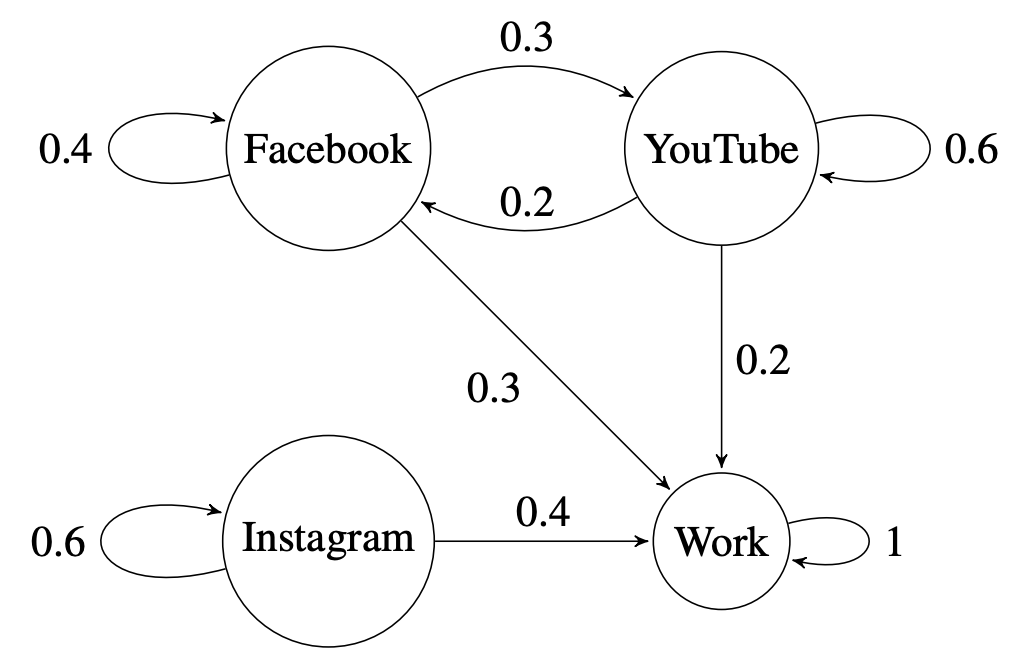
\includegraphics[scale=0.25]{markov_chain}
    \end{figure}
   \begin{enumerate}
       \item Let us define $x_F[n]$ as the number of students on Facebook at timestep $n, x_Y[n]$ as the number of students on YouTube at timestep $n, x_I[n]$ as the number of students on Instagram at timestep $n$, and $x_W[n]$ as the number of students working at timestep $n$. Let the state vector be: $\vec x[n] = \begin{bmatrix}
                                        x_F[n] \\
                                        x_Y[n] \\
                                        x_I[n] \\
                                        x_W[n]    
                                    \end{bmatrix}
       $. Derive the corresponding transition matrix.
    \begin{Answer}
        ...
    \end{Answer}
    
    
    \item There are 1500 of you in the class. Suppose on a given Friday evening (the day when HW is due), there are 700 EECS16A students on Facebook, 450 on YouTube, 200 on Instagram, and 150 actually doing work. In the next timestep, how many people will be doing each activity? In other words, after you apply the matrix once to reach the next timestep, what is the state vector?
    \begin{Answer}
        ...
    \end{Answer}
    
    
    \item Compute the sum of each column in the state transition matrix. What is the interpretation of this?
    \begin{Answer}
        ...
    \end{Answer}
   \end{enumerate}
   
   
   \newpage
   \item $\textbf{Homework Process and Study Group}$
        Who did you work with on this homework? List names and student ID’s. (In case you met people at homework party or in office hours, you can also just describe the group.) How did you work on this homework? If you worked in your study group, explain what role each student played for the meetings this week.
        
        \begin{Answer}
            
        \end{Answer}
    \end{enumerate}


\newpage

\end{document}